% !TEX root = ../main.tex
\section{Neural networks}
\subsection{In silico neural networks}
Artificial neural networks (referred to just as neural networks) is a software implementation of the connection of neurons in the brain. In computer science they can be used to solve a wide variety of problems, like character and facial recognition. They present an advantage over conventional programmatic methods, as they don't need explicit coding for each new problem. There exist many different implementations of neural networks, but in the case of the perceptron (also known as feed-forward neural network), it only needs to know the inputs and the matching outputs to train itself. An example usage showing character recognition can be seen in figure \ref{neuralnetwork_example}.

\begin{figure}[H]
\centering
\includegraphics[width=\columnwidth]{images/neuralnetwork_example.png}
\caption{An example usage of a neural network recognizing the handdrawn letter "a". The typical approach is to segment the area into a grid. Only 2x2 is shown here for simplification, but usually larger grids are used. The average color of each segment is calculated, and fed into a neural network, which has been trained to output "a", when presented an input resembling the handdrawn version.}
\label{neuralnetwork_example}
\end{figure}

The neural network works by simulating the functionality of the brain, by connecting neurons together by varying strength. Continuing the example from figure \ref{neuralnetwork_example}, the 4 segments are fed into 4 input neurons (see figure \ref{neuralnetwork_neurons}). The 4 input neurons are connected to an output neuron by varying strength, much like the synapses of the natural neuron. If the weighted inputs sum exceed the threshold of the output neuron, it will activate. In this simplified example, the output neurons activation is of limited value, as it can only give a yes or no answer to if the input resembles an "a".

\begin{figure}[H]
\centering
\includegraphics[width=200]{images/neuralnetwork_neurons.png}
\caption{}
\label{neuralnetwork_neurons}
\end{figure}

 In a more practical example, the network would have enough input neurons to accommodate a 100x100 grid (10,000 input neurons), have some layers of neurons between the input and output (hidden layers), and enough output neurons to represent binary encoded characters (see figure \ref{neuralnetwork_ocr}).

 \begin{figure}[H]
 \centering
 \includegraphics[width=\columnwidth]{images/neuralnetwork_ocr.png}
 \caption{}
 \label{neuralnetwork_ocr}
 \end{figure}

\subsection{In vitro neural networks}
It has previously been shown that the function of the artificial neuron can also be implemented using strand displacement reactions. The system is based on the seesaw gate motif \cite{Qian}, and can fullfill most of the functionality of a real neuron \cite{Qian2011}.

%INSERT GENERAL INFORMATION ABOUT THE SEESAW WITH TOEHOLDS HERE

\subsubsection{Seesaw gate}

The seesaw gate is a catalytic gate with a threshold, designed for use in scalable strand displacement circuits.


ALSO A SUMMARY OF INPUT WEIGHT, SUMMATION, THRESHOLDING

\subsubsection{Thresholding}
In the natural neuron, the neuron will activate when its inputs exceeds a threshold. This is implemented using a threshold gate which will bind the input and prevent it from reacting downstream in the network. If the threshold gate concentration is higher than the input concentration, the input will be suppressed by the threshold. If the threshold gate concentration is lower than the input concentration, not all of the input is suppressed, and will be able to react further downstream in the network.

% \begin{subfigure}{.49\columnwidth}
%   \centering
%   \includegraphics[width=\linewidth]{images/transcription_annealed_nostain.png}
%   \caption{Not stained}
% \end{subfigure}

\begin{figure}[H]
  \begin{subfigure}[t]{.49\columnwidth}
    \centering
\adjustbox{width=\linewidth} {
% !TEX root = ../main.tex

\begin{tikzpicture}[baseline=-110pt]

\def\inputstrand(#1,#2){
  \begin{scope}[shift={(#1,#2)}]
    \draw[-|](0, 0) -- node[above] {$S_1$} (2, 0);
    \draw[-|](2, 0) -- node[above] {$T$} (3, 0);
    \draw[->](3, 0) -- node[above] {$S_2$} (5, 0);
  \end{scope}
}

% \node at (6, 0) {$+$};

\def\thresholdbot(#1,#2){
  \begin{scope}[shift={(#1,#2)}]
    \draw[<-](7, -0.1) -- node[below] {$s_1^*$} (8, -0.1);
    \draw[|-](8, -0.1) -- node[below] {$T^*$} (9, -0.1);
    \draw[|-](9, -0.1) -- node[below] {$S_2^*$} (11, -0.1);
  \end{scope}
}

\def\thresholdtop(#1,#2){
  \begin{scope}[shift={(#1,#2)}]
    \draw[->](9, 0.1) -- node[above] {$S_2$} (11, 0.1);
  \end{scope}
}

\inputstrand(0,0)
\thresholdbot(0,0)
\thresholdtop(0,0)

\draw[->](6, -2) -- (6, -4);

\inputstrand(0,-5)
\thresholdbot(-6,-5.1)
% \node at (6, -5.1) {$+$};
\thresholdtop(-1,-5.2)

\node[align=center] at (2.5, -1.5) {Input strand};

\node[align=center] at (9, -1.5) {Threshold gate};

\node[align=center] at (9, -6) {Waste};

% \def\strandtwo(#1,#2){
%   \begin{scope}[shift={(#1,#2)}]
%     \draw[<-](4,0.3) -- node[above] {d} (5.9,0.3);
%     \node[label=above:{e}] at (6,1) {};
%     \draw plot [smooth, tension=1] coordinates {(5.9, 0.3) (5.9, 0.4) (5.7, 0.7) (6, 1) (6.3, 0.7) (6.1, 0.4) (6.1, 0.3)};
%     \draw(6.1,0.3) -- node[above] {f} (8,0.3);
%   \end{scope}
% }

\end{tikzpicture}

}
\caption{Reaction of an input strand with a threshold gate. The product has no free toehold domain, and can't undergo reverse reaction. The waste has no toehold, and can't parcitipate in further reactions.}
\label{}
\end{subfigure}
\hfill
\begin{subfigure}[t]{.49\columnwidth}
  \centering
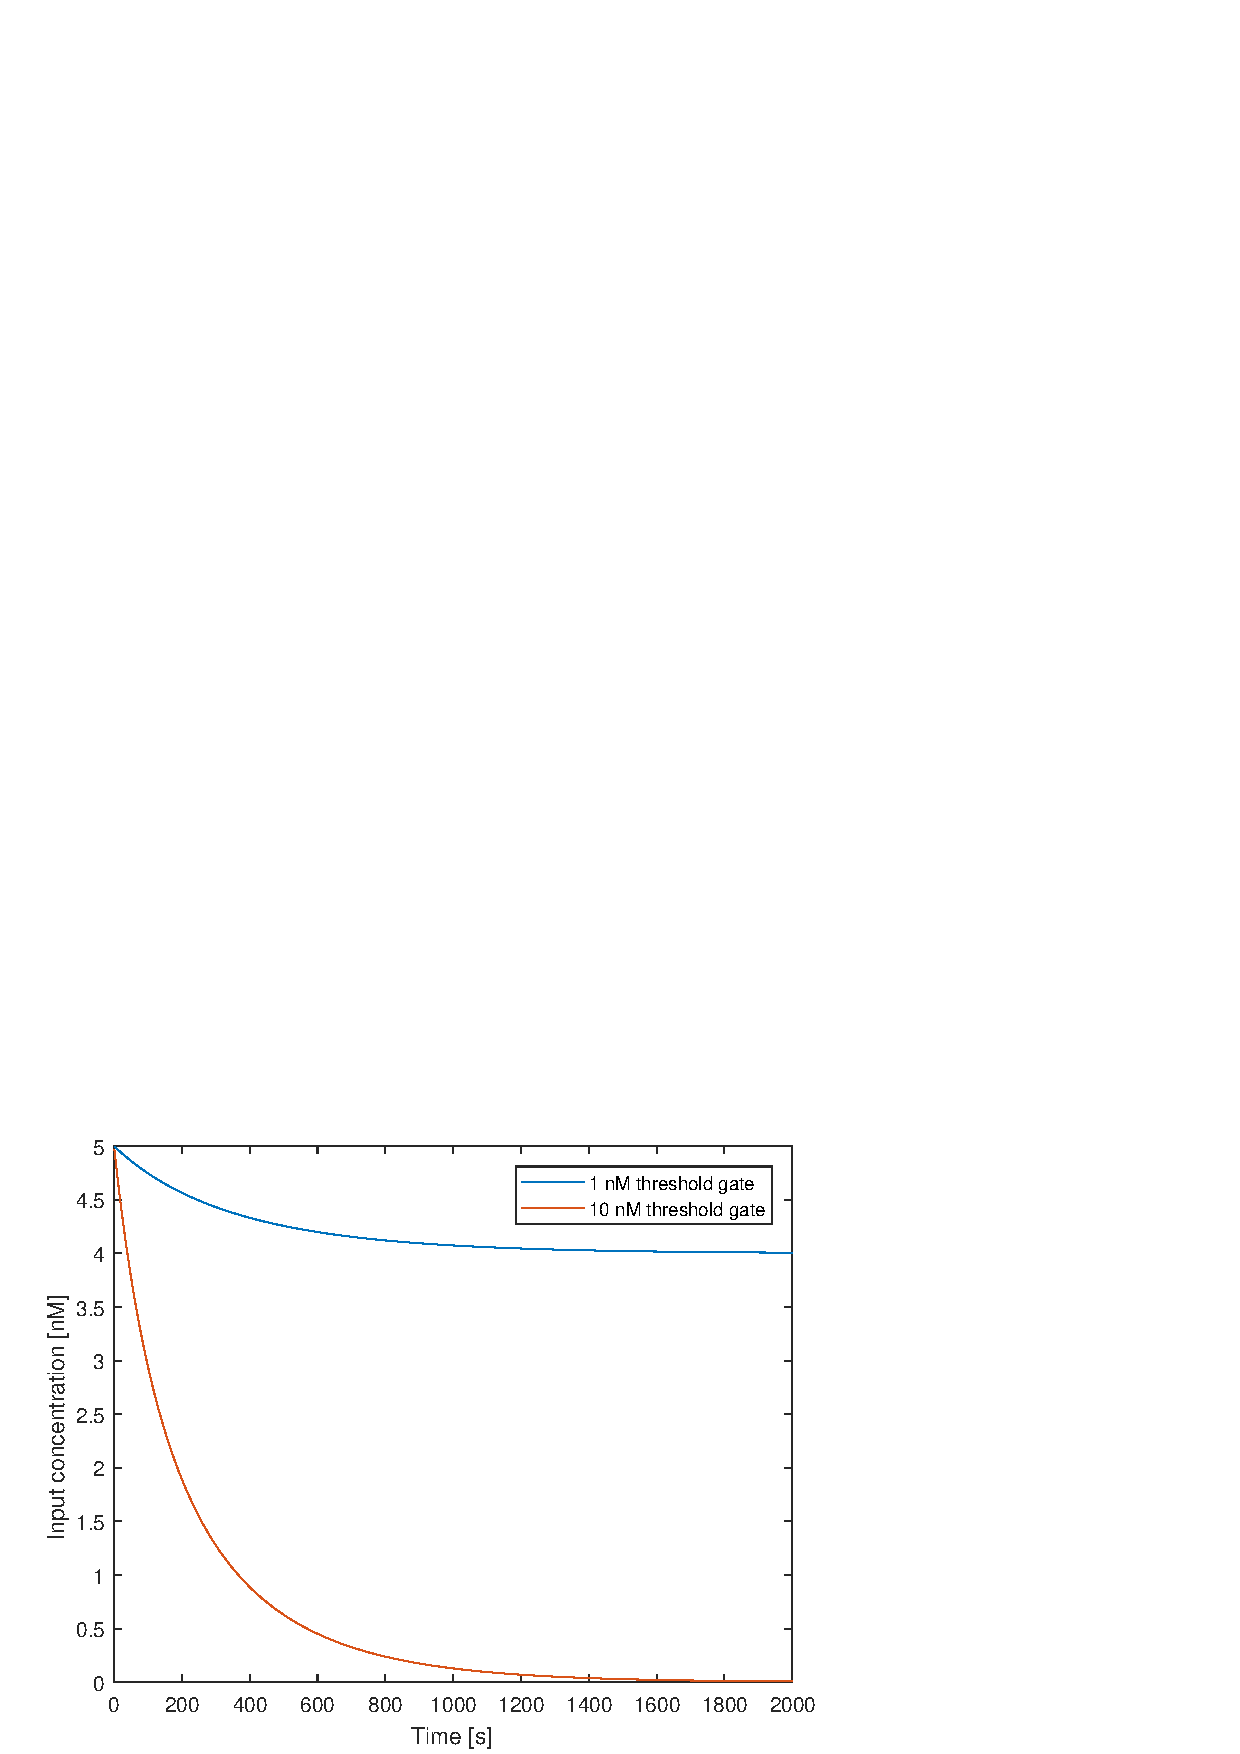
\includegraphics[width=\linewidth]{images/thresholding.png}
\caption{Time analysis of the concentration of input strand (5 nM start concentration). A threshold concentration higher than the input (red) will bind all input strand. A lower concentration (blue), will allow the input strand to participate in further displacement reactions.}
\label{}
\end{subfigure}
\end{figure}

\subsubsection{Integration}
The input to the neuron have to be collected before thresholding, as they don't have the same left recognition sequence. This is done through an integrating gate, which will collect all inputs with the same right recognition sequence, and release a common signal which can be thresholded.

\begin{figure}[H]
  \begin{subfigure}[t]{.49\columnwidth}
    \centering
\adjustbox{width=\linewidth} {
% !TEX root = ../main.tex

\begin{tikzpicture}[baseline=-80pt]

\draw[-|](0, 0) -- node[above] {$S_1$} (2, 0);
\draw[-|](2, 0) -- node[above] {$T$} (3, 0);
\draw[->](3, 0) -- node[above] {$S_2$} (5, 0);

\draw[-|](0, -3) -- node[above] {$S_3$} (2, -3);
\draw[-|](2, -3) -- node[above] {$T$} (3, -3);
\draw[->](3, -3) -- node[above] {$S_2$} (5, -3);

\node at (6, -1.7) {$+$};

\draw[-|](8, -1.5) -- node[above] {$S_2$} (10, -1.5);
\draw[-|](10, -1.5) -- node[above] {$T$} (11, -1.5);
\draw[->](11, -1.5) -- node[above] {$S_4$} (13, -1.5);

\draw[<-](7, -1.7) -- node[below] {$T^*$} (8, -1.7);
\draw[-|](8, -1.7) -- node[below] {$S_2^*$} (10, -1.7);
\draw[-|](10, -1.7) -- node[below] {$T^*$} (11, -1.7);

\node[align=center] at (2.5, -1) {Input 1};

\node[align=center] at (2.5, -4) {Input 2};

\node[align=center] at (10, -3.3) {Integration gate};

\node[align=center] at (10.5, 0) {Output};

\end{tikzpicture}

}
\caption{Reaction of 2 input strands with an integration gate. The input strands have the same right recognition sequence $S_2$, and will both displace the top strand of the integration gate, releasing the output.}
\label{}
\end{subfigure}
\hfill
\begin{subfigure}[t]{.49\columnwidth}
  \centering
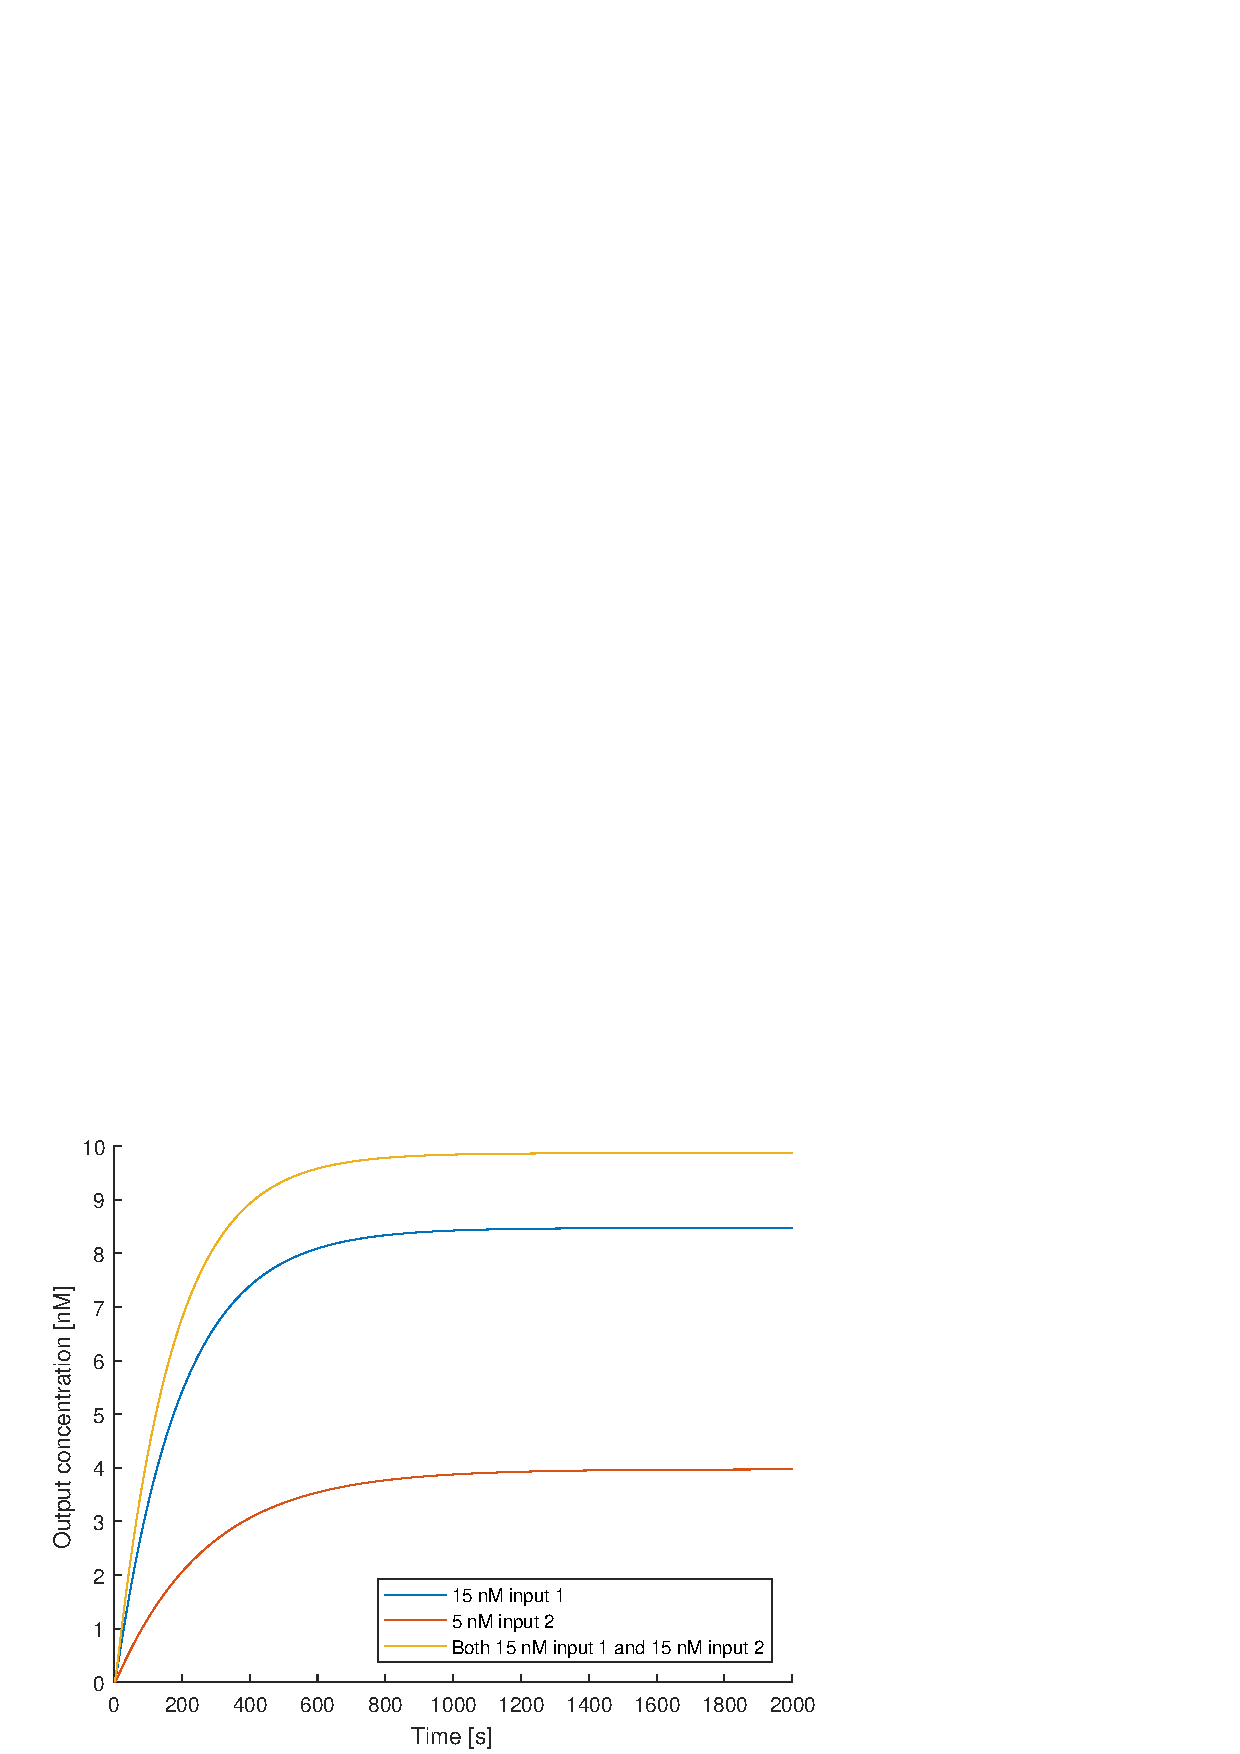
\includegraphics[width=\linewidth]{images/integration.png}
\caption{Time analysis of the concentration of the output strand. The concentration of the integration gate is 20 nM. The first input of 15 nM increases the output strand concentration, compared to the second input of 5 nM. When both strands are added the concentration of output increases further.}
\label{}
\end{subfigure}
\label{seesaw_integration}
\end{figure}

\subsubsection{Weighting}
The inputs to the gate are weighted using their concentration. By making the integration gates concentration the sum of all the input concentrations, a high concentration of one input strand will contribute more to the activation than that of a low concentration, as shown in \fref{seesaw_integration}.

The weight is decided by the concentration of output of a input neuron and its fuel strand. The fuel serves the purpose of pushing the output of one gate to its target concentration.

\begin{figure}[H]
  \begin{subfigure}[t]{.49\columnwidth}
    \centering
\adjustbox{width=\linewidth} {
% !TEX root = ../main.tex

\begin{tikzpicture}[baseline=-250pt]

\def\inputstrand(#1,#2){
  \begin{scope}[shift={(#1,#2)}]
    \draw[-|](0, 0) -- node[above] {$S_1$} (2, 0);
    \draw[-|](2, 0) -- node[above] {$T$} (3, 0);
    \draw[->](3, 0) -- node[above] {$S_2$} (5, 0);
  \end{scope}
}


\def\gatetop(#1,#2){

  \begin{scope}[shift={(#1,#2)}]
\draw[-|](1, -1.5) -- node[above] {$S_2$} (3, -1.5);
\draw[-|](3, -1.5) -- node[above] {$T$} (4, -1.5);
\draw[->](4, -1.5) -- node[above] {$S_3$} (6, -1.5);
\end{scope}
}

\def\gatebottom(#1,#2){

  \begin{scope}[shift={(#1,#2)}]
\draw[<-](0, -1.7) -- node[below] {$T^*$} (1, -1.7);
\draw[|-](1, -1.7) -- node[below] {$S_2^*$} (3, -1.7);
\draw[|-](3, -1.7) -- node[below] {$T^*$} (4, -1.7);
\end{scope}
}

\def\fuel(#1,#2){

  \begin{scope}[shift={(#1,#2)}]
\draw[-|](0, -3) -- node[above] {$S_2$} (2, -3);
\draw[-|](2, -3) -- node[above] {$T$} (3, -3);
\draw[->](3, -3) -- node[above] {$S_f$} (5, -3);
\end{scope}
}

\inputstrand(0,0)
\gatetop(-0.5,-1)
\gatebottom(-0.5,-1)
\fuel(0,-2)

\node[align=center] at (2.5, -0.5) {Input};
%
\node[align=center] at (2.5, -3.5) {Gate};

\node[align=center] at (2.5, -5.5) {Fuel};
\node[align=center] at (13, -3) {Output};
%
% \node[align=center] at (10, -2.7) {Integration gate};
%
% \node[align=center] at (10.5, -0.7) {Output};


\draw[->](7.5, -2.5) -- (8.5, -2.5);

\inputstrand(10,0)
\gatebottom(12,1.5)
\gatetop(9.5,-1)
\gatebottom(10,-3)
\fuel(11,-1.5)

\end{tikzpicture}

}
\caption{Reaction of 2 input strands with an integration gate. The input strands have the same right recognition sequence $S_2$, and will both displace the top strand of the integration gate, releasing the output.}
\label{}
\end{subfigure}
\hfill
\begin{subfigure}[t]{.49\columnwidth}
  \centering
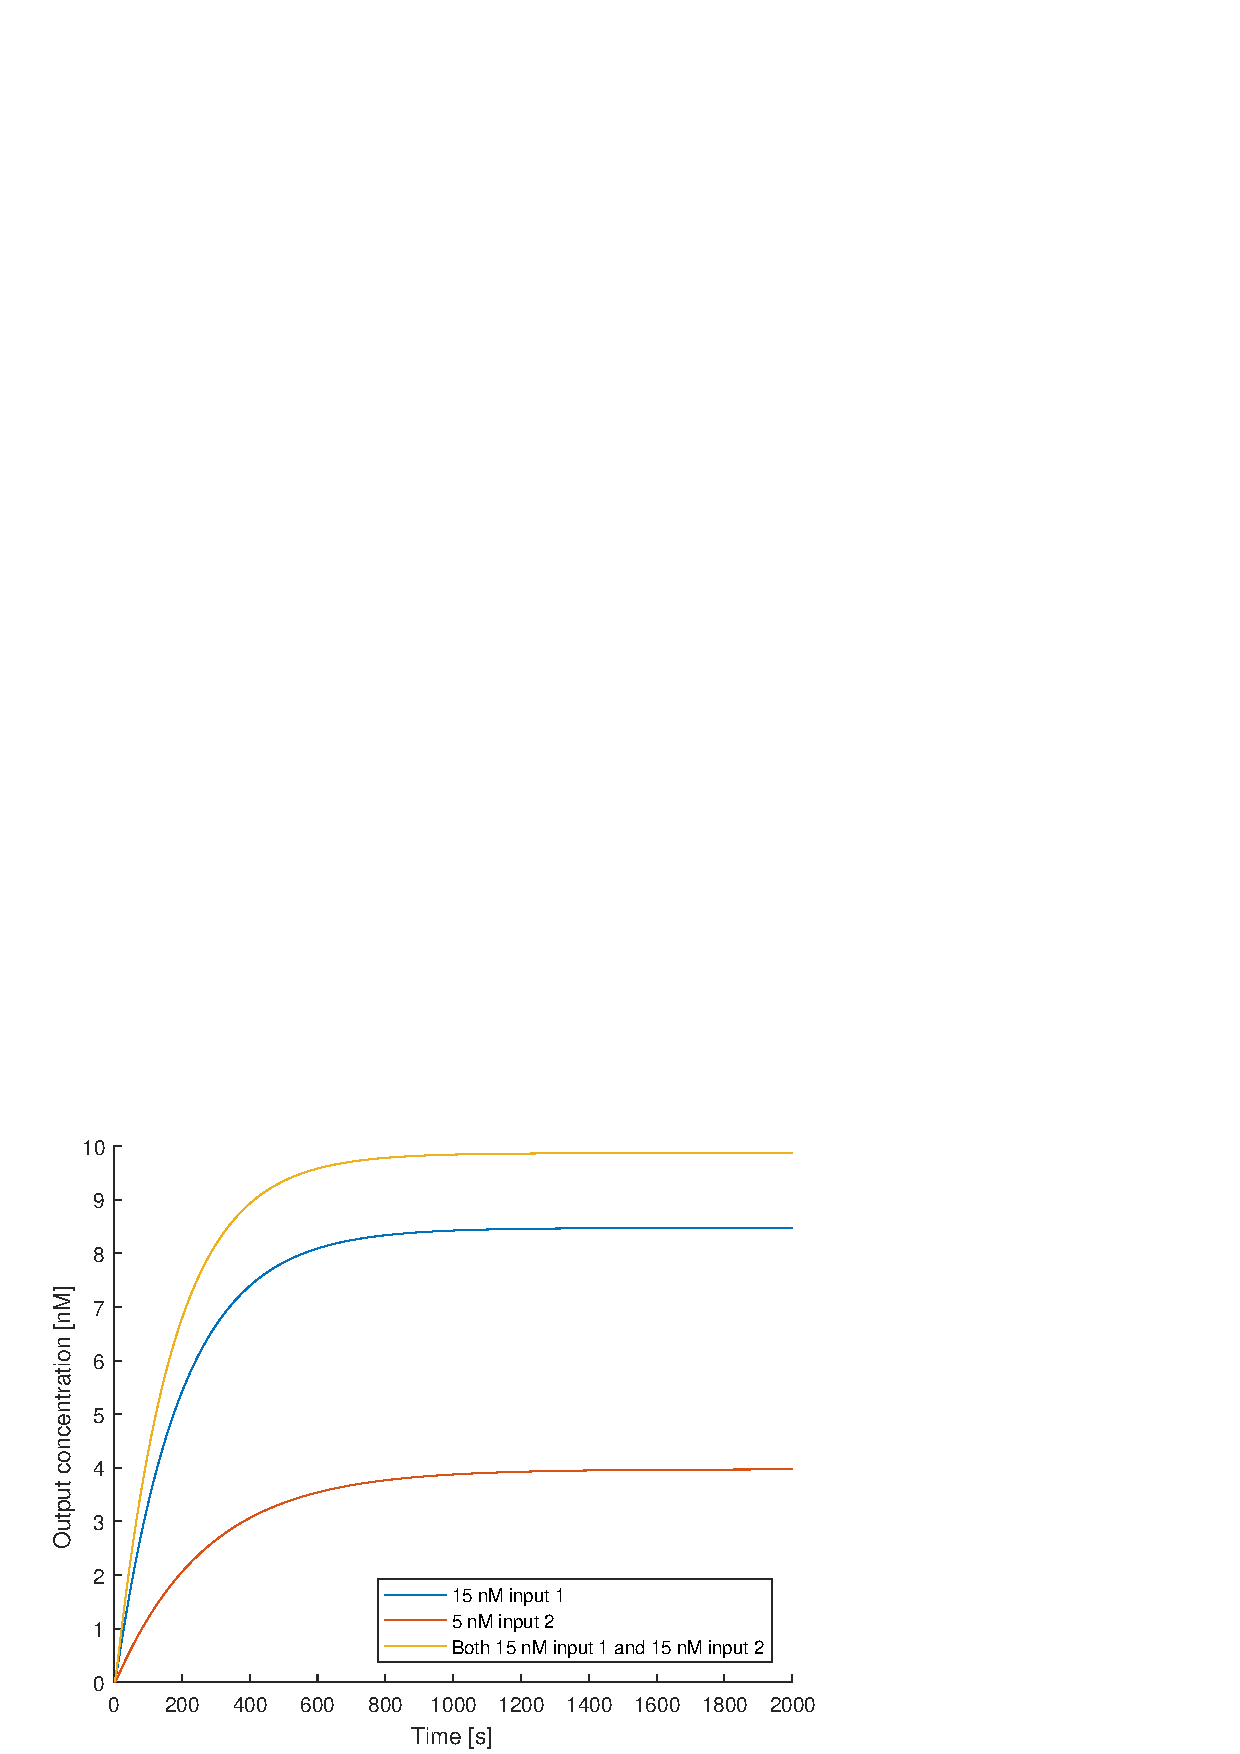
\includegraphics[width=\linewidth]{images/integration.png}
\caption{Time analysis of the concentration of the output strand. The concentration of the integration gate is 20 nM. The first input of 15 nM increases the output strand concentration, compared to the second input of 5 nM. When both strands are added the concentration of output increases further.}
\label{}
\end{subfigure}
\label{seesaw_integration}
\end{figure}

\begin{figure}[H]
\centering
\includegraphics[width=\columnwidth]{images/seesaw_weight.png}
\caption{}
\label{seesaw_weight}
\end{figure}

A problem with this approach to weighting, is that the inputs can only contribute positively to the sum. In silico neural networks can use negative weights to simulate inhibitory synaptic connections, and is needed to implement many kind of boolean functions. The in vitro network can't have negative concentrations of input sequences, so other approaches have to be considered.

WRITE STUFF ABOUT DUAL RAIL LOGIC HERE

\subsubsection{Training}
WRITE STUFF ABOUT TRAINING
